%Author's template: Jose Manuel Vicent-Luna

%Download site: https://github.com/jmviclun/Thesis-LaTeX-Template

%Template for thesis in b5paper format-size. Format adapted from University of Bristol Thesis Template by Victor F. Breña-Medina (https://www.overleaf.com/latex/templates/university-of-bristol-thesis-template/kzqrfvyxxcdm#.WpanyOYrPrd) 

\RequirePackage[l2tabu]{nag}

\documentclass[b5paper,10pt,reqno,openbib]{memoir}

% Memoir is a flexible class for typesetting poetry, fiction, 
% non-fiction and mathematical works as books, reports, articles or
% manuscripts. CTAN repository is found at:
% http://www.ctan.org/tex-archive/macros/latex/contrib/memoir/

\usepackage{datetime}
\usepackage{ifpdf}
\ifpdf
\pdfinfo{
   /Author (Author's name)
   /Title (PhD Thesis)
   /Keywords (kw1; kw2; kw3)
   /CreationDate (D:\pdfdate)
}
\fi
\ifdraftdoc 
\usepackage{draftwatermark} 
\SetWatermarkScale{0.3}
\SetWatermarkText{\bf Draft: \today}
\fi

\newsubfloat{figure}
\newsubfloat{table}
\settrimmedsize{170mm}{240mm}{*}
\setlength{\trimtop}{0pt} 
\setlength{\trimedge}{\stockwidth} 
\addtolength{\trimedge}{-\paperwidth} 
\settypeblocksize{634pt}{448.13pt}{*} 
\setulmargins{4cm}{*}{*} 
\setlrmargins{*}{*}{1.5} 
\setmarginnotes{17pt}{51pt}{\onelineskip} 
\setheadfoot{\onelineskip}{2\onelineskip} 
\setheaderspaces{*}{2\onelineskip}{*} 
%\checkandfixthelayout
\frenchspacing
\usepackage{fouriernc}
\usepackage[T1]{fontenc}
\OnehalfSpacing 
\setsecnumdepth{subsection} 
\maxsecnumdepth{subsubsection}

\usepackage[papersize={170mm,240mm},tmargin=30mm,bmargin=15mm,lmargin=22.5mm,
rmargin=17.5mm]{geometry} 

\usepackage{fancybox}
\usepackage{fancyhdr}
\usepackage{titlesec}

\usepackage{calc,soul,fourier}
\makeatletter 
\newlength\dlf@normtxtw 
\setlength\dlf@normtxtw{\textwidth} 
\newsavebox{\feline@chapter} 
\newcommand\feline@chapter@marker[1][4cm]{%
\sbox\feline@chapter{% 
\resizebox{!}{#1}{\fboxsep=1pt%
\colorbox{gray}{\color{white}\thechapter}% 
}}%
\rotatebox{90}{% 
\resizebox{%
\heightof{\usebox{\feline@chapter}}+\depthof{\usebox{\feline@chapter}}}% 
{!}{\scshape\so\@chapapp}}\quad%
\raisebox{\depthof{\usebox{\feline@chapter}}}{\usebox{\feline@chapter}}%
} 
\newcommand\feline@chm[1][4cm]{%
\sbox\feline@chapter{\feline@chapter@marker[#1]}% 
\makebox[0pt][c]{% aka \rlap
\makebox[0cm][r]{\usebox\feline@chapter}%
}}


%Define two chapter's styles

\makechapterstyle{chapterstyle1}{
\renewcommand\chapnamefont{\normalfont\Large\scshape\raggedleft\so} 
\renewcommand\chaptitlefont{\Large\bfseries}%\scshape} 
\renewcommand\chapternamenum{} \renewcommand\printchaptername{} 
\renewcommand\printchapternum{\null\vskip -100pt\hfill\feline@chm[3.0cm]\par}
%\renewcommand\printchapternum{\null\hfill\feline@chm[3.0cm]\par}
\renewcommand\afterchapternum{\par\vskip\midchapskip} 
\renewcommand\printchaptertitle[1]{\color{gray}\chaptitlefont##1\par}
} 

\makechapterstyle{chapterstyle2}{
\renewcommand\chapnamefont{\normalfont\Large\scshape\raggedleft\so} 
\renewcommand\chaptitlefont{\Large\bfseries}%\scshape} 
\renewcommand\chapternamenum{} \renewcommand\printchaptername{} 
\renewcommand\printchapternum{}
%\renewcommand\printchapternum{\null\hfill\feline@chm[3.0cm]\par}
\renewcommand\afterchapternum{\par\vskip\midchapskip} 
\renewcommand\printchaptertitle[1]{\color{gray}\chaptitlefont##1\par}
}

\patchcmd{\@makechapterhead}{50\p@}{\chapheadtopskip}{}{}
\patchcmd{\@makeschapterhead}{50\p@}{\chapheadtopskip}{}{}
\newlength{\chapheadtopskip}\setlength{\chapheadtopskip}{10pt}

%Define two page's styles

\fancypagestyle{style1}{
\fancyhf{}	
\fancyhead[RO,LE]{\colorbox{gray}{\textbf{\color{white}\thepage}}} 
%\fancyhead[RO,LE]{\thepage} 
%\fancyhead[LO]{\leftmark} 
\fancyhead[RE,LO]{\textbf{Chapter \thechapter}}
%\fancyhead[RE,LO]{\rightmark}
\renewcommand{\headrulewidth}{1.5pt}
}

\fancypagestyle{style2}{
\fancyhf{}	
\fancyhead[RO,LE]{\colorbox{gray}{\textbf{\color{white}\thepage}}} 
%\fancyhead[RO,LE]{\thepage} 
%\fancyhead[LO]{\leftmark} 
\fancyhead[RE,LO]{\textbf{Appendix \thechapter}}
%\fancyhead[RE,LO]{\rightmark}
\renewcommand{\headrulewidth}{1.5pt}
}

\newcommand{\clearemptydoublepage}{\newpage{\thispagestyle{empty}
\cleardoublepage}}
\makeindex

%%%%%%%%%%%%%%%%%%%%%%%%%%%%%%%%%%%%%%%%%%%%%%%%%%%%%%%%%%%%%%%%
%%%%%%%%%%%%%%%%%%%%%%%%%%%%%%%%%%%%%%%%%%%%%%%%%%%%%%%%%%%%%%%%
%%%%%%%%%%%%%%%%%%%%%%%%%%%%%%%%%%%%%%%%%%%%%%%%%%%%%%%%%%%%%%%%
%%%%%%%%%%%%%%%%%%%%%%%%%%%%%%%%%%%%%%%%%%%%%%%%%%%%%%%%%%%%%%%%

%Define packages

\usepackage{import}
\usepackage{lipsum} %Needed to create dummy text
\usepackage{amsfonts} %Calls Amer. Math. Soc. (AMS) fonts
\usepackage[centertags]{amsmath} %Writes maths centred down
\usepackage{stmaryrd} %New AMS symbols
\usepackage{amssymb} %Calls AMS symbols
\usepackage{amsthm} %Calls AMS theorem environment
\usepackage{newlfont} %Helpful package for fonts and symbols
\usepackage{layouts} %Layout diagrams
\usepackage{graphicx} %Calls figure environment
\usepackage{longtable,rotating} %Long tab environments including rotation. 
\usepackage{inputenc} %Needed to encode non english characters 
\usepackage{colortbl} %Makes coloured tables
\usepackage{wasysym} %More math symbols
\usepackage{mathrsfs} %Even more math symbols
\usepackage{float} %Helps to place figures, tables, etc. 
\usepackage{verbatim} %Permits pre-formated text insertion
\usepackage{upgreek } %Calls other kind of greek alphabet
\usepackage{latexsym} %Extra symbols
\usepackage[square,numbers,sort&compress,sectionbib]{natbib} %Calls 
%bibliographycommands
\usepackage{chapterbib}
%\usepackage[style=alphabetic,backend=bibtex]{biblatex}
\usepackage{url} %Supports url commands
\usepackage{etex} %eTeXÕs extended support for counters
\usepackage{fixltx2e}
\usepackage[english]{babel}%For languages characters and hyphenation
\usepackage{color} %Creates coloured text and background
\usepackage[colorlinks=true,allcolors=black]{hyperref}          
%Creates hyperlinks in cross references
\usepackage{memhfixc} %Should be used after hyperref
\usepackage{enumerate} %For enumeration counter
\usepackage{footnote} %For footnotes
\usepackage{microtype} %Makes pdf look better.
\usepackage{rotfloat}
\usepackage{alltt}
\usepackage{multicol}
\usepackage{etoolbox}
\usepackage{relsize}
\usepackage{pdfpages}
%\usepackage{biblatex}
\usepackage{adjustbox}
\setlength{\columnsep}{0.5cm}
\usepackage[version=0.96]{pgf} %PGF/TikZ is a tandem of 
%languages for producing vector graphics from a 
\usepackage{tikz}
%geometric/algebraic description.
\usetikzlibrary{arrows,shapes,snakes,
automata,backgrounds,
petri,topaths}%To use diverse features 

\widowpenalty=1000
\clubpenalty=1000

\usepackage{lettrine}
\usepackage{wrapfig}


%%%%%%%%%%%%%%%%%%%%%%%%%%%%%%%%%%%%%%%%%%%%%%%%%%%%%%%%%%%%%%%%
%%%%%%%%%%%%%%%%%%%%%%%%%%%%%%%%%%%%%%%%%%%%%%%%%%%%%%%%%%%%%%%%
%%%%%%%%%%%%%%%%%%%%%%%%%%%%%%%%%%%%%%%%%%%%%%%%%%%%%%%%%%%%%%%%
%%%%%%%%%%%%%%%%%%%%%%%%%%%%%%%%%%%%%%%%%%%%%%%%%%%%%%%%%%%%%%%%

%Define formats

\newcommand{\initial}[1]{%
\lettrine[lines=3,lhang=0.33,nindent=0em]{
\color{gray}
{\textsc{#1}}}{}}

\newcounter{cnt}\setcounter{cnt}{0}
\def\t{\stepcounter{cnt}\thecnt. cat sat on the mat. }

\newdimen\tttaa
\newdimen\tttbb

\makeatletter
\def\merge@ps{\afterassignment\merge@ps@\tttbb}

\def\merge@ps@{\afterassignment\merge@ps@@\tttaa}

\def\merge@ps@@{%
\afterassignment\reset@WF@ps\dimen@\WF@ps\valign
%\showthe\count@
\ifnum\count@>\@ne
\advance\count@\m@ne
\expandafter\merge@ps
\fi
}

\def\reset@WF@ps{\afterassignment\reset@WF@ps@\dimen@ii}

\def\reset@WF@ps@#1\valign{%
\edef\new@wf@ps{\new@wf@ps
  \the\dimexpr\dimen@+\tttbb\relax\space
  \the\dimexpr\dimen@ii-\tttbb\relax\space}%
 \def\WF@ps{#1}}

\newcommand{\wflettrine}[3][]{%
  
\setbox\tw@\hbox{\lettrine[#1]{#2}{#3}\global\let\gtmp\L@parshape}%
  \afterassignment\wf@getoffset\count@\gtmp\hoffset
  \setbox\WF@box\hbox{\kern-\dimen@\box\WF@box\kern\dimen@}%
  \noindent\box\tw@
    \def\new@wf@ps{}%
    \afterassignment\merge@ps\count@\gtmp
    \edef\WF@ps{\new@wf@ps\space\WF@ps}%
    \@@parshape\c@WF@wrappedlines\WF@ps\z@\columnwidth}

\def\wf@getoffset{\afterassignment\wf@get@ffset\dimen@}
\def\wf@get@ffset#1\hoffset{}

\makeatother

\makeatletter
\renewcommand{\@memb@bchap}{%
  \section*{\bibname}%
  \bibmark
  \ifnobibintoc\else
    \phantomsection
    \addcontentsline{toc}{chapter}{\bibname}%
  \fi
  \prebibhook}
\makeatother

\patchcmd{\mcitethebibliography}
  {\advance\leftmargin\labelsep}
  {\leftmargin=0pt\itemindent=\labelwidth\advance\itemindent\labelsep}
  {}{}


%%%%%%%%%%%%%%%%%%%%%%%%%%%%%%%%%%%%%%%%%%%%%%%%%%%%%%%%%%%%%%%%
%%%%%%%%%%%%%%%%%%%%%%%%%%%%%%%%%%%%%%%%%%%%%%%%%%%%%%%%%%%%%%%%
%%%%%%%%%%%%%%%%%%%%%%%%%%%%%%%%%%%%%%%%%%%%%%%%%%%%%%%%%%%%%%%%
%%%%%%%%%%%%%%%%%%%%%%%%%%%%%%%%%%%%%%%%%%%%%%%%%%%%%%%%%%%%%%%%
  
  
%% Define user's commands  
\newcommand{\cod}{CO$_2$\,}
\newcommand{\chc}{CH$_4$\,}
\newcommand{\nd}{N$_2$\,}
  
%choose default chapter and page styles

\makeatother 
\chapterstyle{chapterstyle1}
\pagestyle{style1}	

%%%%%%%%%%%%%%%%%%%%%%%%%%%%%%%%%%%%%%%%%%%%%%%%%%%%%%%%%%%%%%%%
%%%%%%%%%%%%%%%%%%%%%%%%%%%%%%%%%%%%%%%%%%%%%%%%%%%%%%%%%%%%%%%%
%%%%%%%%%%%%%%%%%%%%%%%%%%%%%%%%%%%%%%%%%%%%%%%%%%%%%%%%%%%%%%%%
%%%%%%%%%%%%%%%%%%%%%%%%%%%%%%%%%%%%%%%%%%%%%%%%%%%%%%%%%%%%%%%%

\begin{document}
% 
\frontmatter
\pagenumbering{roman}

\pagestyle{empty}

\includepdf[pages=1,pagecommand={},offset=-6.7cm 
-0.5cm]{frontmatter/cover_thesis_front.pdf}
\clearemptydoublepage

%%
% file: blank.tex
% author: José Manuel Vicent Luna
% description: Contains a blank page for the beginning
%

\thispagestyle{empty}
\phantom{x}
%\clearemptydoublepage


\begin{titlingpage}
\begin{SingleSpace}
\calccentering{\unitlength} 
%\begin{adjustwidth*}{\unitlength}{-\unitlength}
\begin{adjustwidth*}{-0.5cm}{0.5cm}
\vspace*{5mm}
\begin{center}
\rule[0.5ex]{\linewidth}{2pt}\vspace*{-\baselineskip}\vspace*{3.2pt}
\rule[0.5ex]{\linewidth}{1pt}\\[\baselineskip]
{\huge title part a\\
\vspace{2mm}
 title part b }\\[4mm]
%{\Large \textit{Subtitle}}\\
\rule[0.5ex]{\linewidth}{1pt}\vspace*{-\baselineskip}\vspace*{4.2pt}
\rule[0.5ex]{\linewidth}{2pt}\\
\vspace{4.5mm}
{\large By}\\
\vspace{4.5mm}
{\large\textbf{\textsc{author name and surname}}}\\
\vspace{2.5mm}
\large{formation }\\
\vspace{9mm}

\includegraphics[scale=0.4]{logos/logo1.jpg}\\
\vspace{4mm}
{\large Department of ...\\
\vspace{2mm}
\textsc{University ...}}\\
\vspace{9mm}
{\Large\textsc{Supervisors}}\\
\vspace{2mm}
name surname\\
\vspace{2mm}
Prof./Dr. University ...\\
\vspace{5mm}
name surname\\
\vspace{2mm}
Prof./Dr. University ...\\
\end{center}
\begin{center}
\vspace{-1mm}
\hspace{0cm} Dissertation submitted to obtain the degree of Doctor with international mention.\\
\vspace{5mm}
{\large\textsc{Place, month year}}
\end{center}
\end{adjustwidth*}
\vspace{12mm}
\begin{flushright}
%{\small Word count: ten thousand and four}
\end{flushright}

\vspace{10cm}

%information and link to personal sites: (optional)


%ISBN: XXX-XX-XXX-XXXX-X \\

%Copyright \textcopyright\,\, author name surname \\


%\begin{wrapfigure}{L}{1.5cm}
%\centering
%\vspace{-0.6cm}
%\includegraphics[width=0.5cm]{logos/logo.png}
%\end{wrapfigure}

%\vspace{0cm}
%\hspace{-1.5cm}
%\href{https://www.site.com/site}{link-text}\\


%\href{https://www.site.com/site}{\includegraphics 
%[scale=0.15]{logos/link-logo.png}}

%\vspace{0.5cm}
%Printed by: printer-site



\end{SingleSpace}
\end{titlingpage}

\clearemptydoublepage


%
% file: funding.tex
% author: Jose Manuel Vicent-Luna
% description: Contains the list of fundings and committee
%


\renewcommand{\labelitemi}{\scriptsize$\blacksquare$}

\noindent \rule{0.6\textwidth}{2.0pt}
\vspace{-0.4cm}

\noindent \rule{0.6\textwidth}{0.5pt}

\begin{itemize}
 \item \textbf{Doctoral Supervisors} 
 
 
  \hspace{0.5cm} Prof./Dr. name surname
  
  \hspace{0.5cm} Prof./Dr. name surname\\
  
  \item \textbf{Examination Committe}
  
  \hspace{0.5cm} Chair: Prof./Dr. name surname
  
  \hspace{0.5cm} Secretary:  Prof./Dr. name surname
  
  \hspace{0.5cm} Member: Prof./Dr. name surname\\
  
  
  \item \textbf{External Committe}
  
  \hspace{0.5cm} Prof./Dr. name surname
  
  \hspace{0.5cm} Prof./Dr. name surname
  
\end{itemize}

\noindent \rule{0.6\textwidth}{0.5pt}
\vspace{-0.35cm}

\noindent \rule{0.6\textwidth}{2.0pt}


\vspace{1.5cm}

\noindent The research reported in this thesis was carried out at ...  with financial support from the ... \\

\begin{figure}[H]
 \centering
 
\includegraphics[scale=0.055]{logos/logo2.png}
 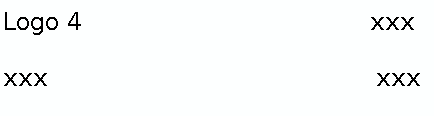
\includegraphics[scale=0.45]{logos/logo4.png}
 
\includegraphics[scale=0.08]{logos/logo3.png}
 \end{figure}







\clearemptydoublepage

\pagestyle{style1}

\renewcommand{\contentsname}{Table of Contents}
\maxtocdepth{subsection}
\tableofcontents*
\addtocontents{toc}{\par\nobreak \mbox{}\hfill{\bf Page}\par\nobreak}
\clearemptydoublepage


\mainmatter


\pagestyle{style1}

% File: chapter-intro.tex
% Author: Jose Manuel Vicent-Luna
%
\chapter{Introduction}

\noindent \rule{\textwidth}{0.5pt}

\begin{wrapfigure}{t}{0cm}
\centering
\includegraphics[width=8cm]{logos/thesisdefense.png}
\end{wrapfigure}
\color{gray}\wflettrine[lines=3]{A}{} \color{black}bstract introduction Lorem ipsum dolor sit amet, consectetur adipiscing elit. Pellentesque ligula mauris, tempor et nunc eu, maximus ullamcorper ligula. Sed mollis convallis lectus in elementum. Fusce at auctor tortor. Sed at ligula lacus. Donec vitae lectus facilisis, maximus risus id, fringilla sapien. Donec sed nibh in metus aliquam congue vel at enim. Aliquam nisl arcu, tristique et varius id, convallis at purus. Vivamus in augue non magna accumsan vestibulum quis in odio. Donec sagittis justo eu ante pharetra vehicula. \\


(Image URL (for hotlinking/embedding):

 https://imgs.xkcd.com/comics/thesis\_defense.png)\\


Morbi faucibus consectetur metus, quis feugiat quam molestie nec. Interdum et malesuada fames ac ante ipsum primis in faucibus. Quisque sollicitudin laoreet elementum. Integer tincidunt massa quis feugiat rutrum. Maecenas auctor vel diam vel rhoncus. Morbi semper lacus diam. 


\noindent \rule{\textwidth}{0.5pt}

\newpage
%=======
\begin{multicols}{2}
\section{\textsc{section1}}
\label{sec:sec01}
\vspace{-0.2cm}
\subsection{subsection1}
\vspace{-0.1cm}

 Lorem ipsum dolor sit amet,\cite{labelcite1} consectetur adipiscing elit. Pellentesque ligula mauris, tempor et nunc eu, maximus ullamcorper ligula. Sed mollis convallis lectus in elementum. Fusce at auctor tortor. Sed at ligula lacus. Donec vitae lectus facilisis, maximus risus id, fringilla sapien. Donec sed nibh in metus aliquam congue vel at enim. Aliquam nisl arcu, tristique et varius id, convallis at purus. Vivamus in augue non magna accumsan vestibulum quis in odio. Donec sagittis justo eu ante pharetra vehicula.

Morbi faucibus consectetur metus,\cite{labelcite1,labelcite3} quis feugiat quam molestie nec. Interdum et malesuada fames ac ante ipsum primis in faucibus. Quisque sollicitudin laoreet elementum. Integer tincidunt massa quis feugiat rutrum. Maecenas auctor vel diam vel rhoncus. Morbi semper lacus diam. Sed quis ligula congue, elementum lorem eget, sodales orci. Sed eu consequat dolor, a posuere elit. Praesent tempor aliquet blandit. Aenean blandit sapien et diam lobortis auctor. Nunc vel neque et nibh fringilla fermentum. 


\begin{figure}[H]
 \begin{center}
\vspace{-0.4cm} 
\includegraphics[width=0.45
\textwidth]{chapters/chapter-intro/fig-intro/thesisdefense.png}
 \end{center}
 \textbf{Figure 1.} \small{Image URL (for hotlinking/embedding):
https://imgs.xkcd.com/comics/thesis\_defense.png}  
\rule{0.49\textwidth}{1.0pt}
\end{figure}


\noindent  Lorem ipsum dolor sit amet, consectetur adipiscing elit. Pellentesque ligula mauris, tempor et nunc eu, maximus ullamcorper ligula. Sed mollis convallis lectus in elementum. Fusce at auctor tortor. Sed at ligula lacus. Donec vitae lectus facilisis, maximus risus id, fringilla sapien. Donec sed nibh in metus aliquam congue vel at enim. Aliquam nisl arcu, tristique et varius id, convallis at purus. Vivamus in augue non magna accumsan vestibulum quis in odio. Donec sagittis justo eu ante pharetra vehicula.

Morbi faucibus consectetur metus, quis feugiat quam molestie nec. Interdum et malesuada fames ac ante ipsum primis in faucibus. Quisque sollicitudin laoreet elementum. Integer tincidunt massa quis feugiat rutrum. Maecenas auctor vel diam vel rhoncus. Morbi semper lacus diam. Sed quis ligula congue, elementum lorem eget, sodales orci. Sed eu consequat dolor, a posuere elit. Praesent tempor aliquet blandit. Aenean blandit sapien et diam lobortis auctor. Nunc vel neque et nibh fringilla fermentum. 



\subsection{subsection2}

 Lorem ipsum dolor sit amet, consectetur adipiscing elit. Pellentesque ligula mauris, tempor et nunc eu, maximus ullamcorper ligula. Sed mollis convallis lectus in elementum. Fusce at auctor tortor. Sed at ligula lacus. Donec vitae lectus facilisis, maximus risus id, fringilla sapien. Donec sed nibh in metus aliquam congue vel at enim. Aliquam nisl arcu, tristique et varius id, convallis at purus. Vivamus in augue non magna accumsan vestibulum quis in odio. Donec sagittis justo eu ante pharetra vehicula.

Morbi faucibus consectetur metus, quis feugiat quam molestie nec. Interdum et malesuada fames ac ante ipsum primis in faucibus. Quisque sollicitudin laoreet elementum. Integer tincidunt massa quis feugiat rutrum. Maecenas auctor vel diam vel rhoncus. Morbi semper lacus diam. Sed quis ligula congue, elementum lorem eget, sodales orci. Sed eu consequat dolor, a posuere elit. Praesent tempor aliquet blandit. Aenean blandit sapien et diam lobortis auctor. Nunc vel neque et nibh fringilla fermentum. 



\section{\textsc{section2}}
\label{sec:sec02}

Section text ...

\subsection{subsection3}

 Lorem ipsum dolor sit amet, consectetur adipiscing elit. Pellentesque ligula mauris, tempor et nunc eu, maximus ullamcorper ligula. Sed mollis convallis lectus in elementum. Fusce at auctor tortor. Sed at ligula lacus. Donec vitae lectus facilisis, maximus risus id, fringilla sapien. Donec sed nibh in metus aliquam congue vel at enim. Aliquam nisl arcu, tristique et varius id, convallis at purus. Vivamus in augue non magna accumsan vestibulum quis in odio. Donec sagittis justo eu ante pharetra vehicula.

Morbi faucibus consectetur metus, quis feugiat quam molestie nec. Interdum et malesuada fames ac ante ipsum primis in faucibus. Quisque sollicitudin laoreet elementum. Integer tincidunt massa quis feugiat rutrum. Maecenas auctor vel diam vel rhoncus. Morbi semper lacus diam. Sed quis ligula congue, elementum lorem eget, sodales orci. Sed eu consequat dolor, a posuere elit. Praesent tempor aliquet blandit. Aenean blandit sapien et diam lobortis auctor. Nunc vel neque et nibh fringilla fermentum. 


\begin{equation} 
\aleph_{NPT}\,\, (V;\vec{s}^N) \propto V^N e^{-\beta PV} e^{-\beta 
U(\vec{s}^N)} 
\end{equation}


\noindent where ...

\begin{equation}
\begin{aligned}
 Z_{NPT}= & \frac{\beta P}{\Lambda^{3N}N!} \int V^N e^{-\beta PV} \times \\ 
& \times \left(\int e^{-\beta U(\vec{s}^N)}d\vec{s}^N\right)dV
 \end{aligned}
\end{equation}



\section{\textsc{Outline of the Thesis}}
\label{sec:sec04}

In this thesis we have ...


 \noindent \textbullet\,\, \textbf{block 1. (Chapters X, and X)}\\ 


\noindent text ...\\

 \noindent \textbullet\,\, \textbf{block 2. (Chapters X, and X)}\\ 


\noindent text ...



\begingroup
    \setlength\bibindent{-20pt}
    \setlength{\bibsep}{0pt}
\scriptsize{\bibliographystyle{../../thisthesisbibliostyle}
\bibliography{../../thesisbiblio}
}
\endgroup



\end{multicols}
%=========================================================

\clearemptydoublepage
%
% File: chapter-template.tex
% Author: Jose Manuel Vicent-Luna
%
\chapter{Chapter title}
\vspace{-0.7cm}


\begin{center}
\textbf{\underline{author 1 name surname}, author 2 name surname, and author 3 
name surname}
\end{center}

\vspace{-0.5cm}

\noindent \rule{\textwidth}{0.5pt}
\vspace{-0.5cm}

\begin{wrapfigure}{t}{0cm}
\centering
\includegraphics[width=7cm] 
{chapters/chapter-template/fig-template/thesisdefense.png}
\end{wrapfigure}
\color{gray}\wflettrine[lines=3]{A}{} \color{black}bstract chapter text
 Lorem ipsum dolor sit amet, consectetur adipiscing elit. Pellentesque ligula 
mauris, tempor et nunc eu, maximus ullamcorper ligula. Sed mollis convallis 
lectus in elementum. Fusce at auctor tortor. Sed at ligula lacus. Donec vitae 
lectus facilisis, maximus risus id, fringilla sapien. Donec sed nibh in metus 
aliquam congue vel at enim. Aliquam nisl arcu, tristique et varius id, convallis 
at purus. Vivamus in augue non magna accumsan vestibulum quis in odio. Donec 
sagittis justo eu ante pharetra vehicula.\\

Image URL (for hotlinking/embedding): 

https://imgs.xkcd.com/comics/thesis\_defense.png\\

Morbi faucibus consectetur metus, quis feugiat quam molestie nec. Interdum et 
malesuada fames ac ante ipsum primis in faucibus. Quisque sollicitudin laoreet 
elementum. 

\noindent \rule{\textwidth}{0.5pt}

%=======
\begin{multicols}{2}
\section{\textsc{Introduction}}
\label{sec:sec01}

Here, the introduction ...




\section{\textsc{Simulation/Experimental Details}}
\label{sec:sec02}

Here the methodology ...

\section{\textsc{Results and Discussion}}
\label{sec:sec03}

Here the results ...\\

 Lorem ipsum dolor sit amet,\cite{labelcite1} consectetur adipiscing elit. Pellentesque ligula 
mauris, tempor et nunc eu, maximus ullamcorper ligula.\cite{labelcite1,labelcite2,labelcite3} Sed mollis convallis 
lectus in elementum. Fusce at auctor tortor. Sed at ligula lacus. Donec vitae 
lectus facilisis, maximus risus id, fringilla sapien. Donec sed nibh in metus 
aliquam congue vel at enim.\cite{labelcite1,labelcite3,labelcite4,labelcite5} Aliquam nisl arcu, tristique et varius id, convallis 
at purus. Vivamus in augue non magna accumsan vestibulum quis in odio. Donec 
sagittis justo eu ante pharetra vehicula.

Morbi faucibus consectetur metus, quis feugiat quam molestie nec. Interdum et 
malesuada fames ac ante ipsum primis in faucibus. Quisque sollicitudin laoreet 
elementum. Integer tincidunt massa quis feugiat rutrum. Maecenas auctor vel diam 
vel rhoncus. Morbi semper lacus diam. Sed quis ligula congue, elementum lorem 
eget, sodales orci. Sed eu consequat dolor, a posuere elit. Praesent tempor 
aliquet blandit. Aenean blandit sapien et diam lobortis auctor. Nunc vel neque 
et nibh fringilla fermentum.\linebreak


\begin{figure}[H]
 \begin{center}
 
\includegraphics[width=0.48\textwidth] 
{chapters/chapter-template/fig-template/thesisdefense.png}
 \end{center}
 \textbf{Figure 1.} \small{Image URL (for hotlinking/embedding): 
https://imgs.xkcd.com/comics/thesis\_defense.png}
\rule{0.49\textwidth}{1.0pt}
\end{figure}

 Lorem ipsum dolor sit amet, consectetur adipiscing elit. Pellentesque ligula 
mauris, tempor et nunc eu, maximus ullamcorper ligula. Sed mollis convallis 
lectus in elementum. Fusce at auctor tortor. Sed at ligula lacus. Donec vitae 
lectus facilisis, maximus risus id, fringilla sapien. Donec sed nibh in metus 
aliquam congue vel at enim. Aliquam nisl arcu, tristique et varius id, convallis 
at purus. Vivamus in augue non magna accumsan vestibulum quis in odio. Donec 
sagittis justo eu ante pharetra vehicula.

Morbi faucibus consectetur metus, quis feugiat quam molestie nec. Interdum et 
malesuada fames ac ante ipsum primis in faucibus. Quisque sollicitudin laoreet 
elementum. Integer tincidunt massa quis feugiat rutrum. Maecenas auctor vel diam 
vel rhoncus. Morbi semper lacus diam. Sed quis ligula congue, elementum lorem 
eget, sodales orci. Sed eu consequat dolor, a posuere elit. Praesent tempor 
aliquet blandit. Aenean blandit sapien et diam lobortis auctor. Nunc vel neque 
et nibh fringilla fermentum. 

 Lorem ipsum dolor sit amet, consectetur adipiscing elit. Pellentesque ligula 
mauris, tempor et nunc eu, maximus ullamcorper ligula. Sed mollis convallis 
lectus in elementum. Fusce at auctor tortor. Sed at ligula lacus. Donec vitae 
lectus facilisis, maximus risus id, fringilla sapien. Donec sed nibh in metus 
aliquam congue vel at enim. Aliquam nisl arcu, tristique et varius id, convallis 
at purus. Vivamus in augue non magna accumsan vestibulum quis in odio. Donec 
sagittis justo eu ante pharetra vehicula.

Morbi faucibus consectetur metus, quis feugiat quam molestie nec. Interdum et 
malesuada fames ac ante ipsum primis in faucibus. Quisque sollicitudin laoreet 
elementum. Integer tincidunt massa quis feugiat rutrum. Maecenas auctor vel diam 
vel rhoncus. Morbi semper lacus diam. Sed quis ligula congue, elementum lorem 
eget, sodales orci. Sed eu consequat dolor, a posuere elit. Praesent tempor 
aliquet blandit. Aenean blandit sapien et diam lobortis auctor. Nunc vel neque 
et nibh fringilla fermentum. 

 Lorem ipsum dolor sit amet, consectetur adipiscing elit. Pellentesque ligula 
mauris, tempor et nunc eu, maximus ullamcorper ligula. Sed mollis convallis 
lectus in elementum. Fusce at auctor tortor. Sed at ligula lacus. Donec vitae 
lectus facilisis, maximus risus id, fringilla sapien. Donec sed nibh in metus 
aliquam congue vel at enim. Aliquam nisl arcu, tristique et varius id, convallis 
at purus. Vivamus in augue non magna accumsan vestibulum quis in odio. Donec 
sagittis justo eu ante pharetra vehicula.

Morbi faucibus consectetur metus, quis feugiat quam molestie nec. Interdum et 
malesuada fames ac ante ipsum primis in faucibus. Quisque sollicitudin laoreet 
elementum. Integer tincidunt massa quis feugiat rutrum. Maecenas auctor vel diam 
vel rhoncus. Morbi semper lacus diam. Sed quis ligula congue, elementum lorem 
eget, sodales orci. Sed eu consequat dolor, a posuere elit. Praesent tempor 
aliquet blandit. Aenean blandit sapien et diam lobortis auctor. Nunc vel neque 
et nibh fringilla fermentum. 

\end{multicols}


\begin{figure}[H]
 \begin{center}
 
\includegraphics[width=0.8\textwidth]
{chapters/chapter-template/fig-template/thesisdefense.png}

 \end{center}
 \textbf{Figure 2.} \small{{Image URL (for hotlinking/embedding): 
https://imgs.xkcd.com/comics/thesis\_defense.png}}
\rule{1.0\textwidth}{1.0pt}
\end{figure}


\begin{multicols}{2}


 Lorem ipsum dolor sit amet, consectetur adipiscing elit. Pellentesque ligula 
mauris, tempor et nunc eu, maximus ullamcorper ligula. Sed mollis convallis 
lectus in elementum. Fusce at auctor tortor. Sed at ligula lacus. Donec vitae 
lectus facilisis, maximus risus id, fringilla sapien. Donec sed nibh in metus 
aliquam congue vel at enim. Aliquam nisl arcu, tristique et varius id, convallis 
at purus. Vivamus in augue non magna accumsan vestibulum quis in odio. Donec 
sagittis justo eu ante pharetra vehicula.

Morbi faucibus consectetur metus, quis feugiat quam molestie nec. Interdum et 
malesuada fames ac ante ipsum primis in faucibus. Quisque sollicitudin laoreet 
elementum. Integer tincidunt massa quis feugiat rutrum. Maecenas auctor vel diam 
vel rhoncus. Morbi semper lacus diam. Sed quis ligula congue, elementum lorem 
eget, sodales orci. Sed eu consequat dolor, a posuere elit. Praesent tempor 
aliquet blandit. Aenean blandit sapien et diam lobortis auctor. Nunc vel neque 
et nibh fringilla fermentum. 

\begin{table}[H]
\rule{0.49\textwidth}{1.0pt}

\noindent \textbf{Table XX-1.} \small{Table title.} 
 \begin{center}
 \begin{adjustbox}{max width=0.49\textwidth}
 \begin{tabular}[c]{lcccc}

  & \multicolumn{4}{c}{\textbf{\Large{XXXX}}} \\
  \vspace{-0.4cm}\\
  & \multicolumn{4}{c}{\rule{35mm}{0.5mm}} \\
  
  \textbf{\Large{XXXX2}} & \textbf{\Large{X3}} & \textbf{\Large{X4}} & 
\textbf{\Large{X5}} & \textbf{\Large{X6}}\\
  \vspace{-10.0pt}\\
  \hline
  \vspace{-10.0pt}\\
  \textbf{c1}     &  v1 & v2  & v3 &  v4 \\
  \textbf{c1}     &  v1 & v2  & v3 &  v4 \\
  \textbf{c1}     &  v1 & v2  & v3 &  v4 \\
  \textbf{c1}     &  v1 & v2  & v3 &  v4 \\
  \vspace{-10.0pt}\\
  \hline
 \end{tabular}
 \end{adjustbox}
 \end{center}
\end{table}


 Lorem ipsum dolor sit amet, consectetur adipiscing elit. Pellentesque ligula 
mauris, tempor et nunc eu, maximus ullamcorper ligula. Sed mollis convallis 
lectus in elementum. Fusce at auctor tortor. Sed at ligula lacus. Donec vitae 
lectus facilisis, maximus risus id, fringilla sapien. Donec sed nibh in metus 
aliquam congue vel at enim. Aliquam nisl arcu, tristique et varius id, convallis 
at purus. Vivamus in augue non magna accumsan vestibulum quis in odio. Donec 
sagittis justo eu ante pharetra vehicula.

Morbi faucibus consectetur metus, quis feugiat quam molestie nec. Interdum et 
malesuada fames ac ante ipsum primis in faucibus. Quisque sollicitudin laoreet 
elementum. Integer tincidunt massa quis feugiat rutrum. Maecenas auctor vel diam 
vel rhoncus. Morbi semper lacus diam. Sed quis ligula congue, elementum lorem 
eget, sodales orci. Sed eu consequat dolor, a posuere elit. Praesent tempor 
aliquet blandit. Aenean blandit sapien et diam lobortis auctor. Nunc vel neque 
et nibh fringilla fermentum. 




\section{\textsc{Conclusions}}
\label{sec:sec04}

Here, the conclusions... 
 Lorem ipsum dolor sit amet, consectetur adipiscing elit. Pellentesque ligula 
mauris, tempor et nunc eu, maximus ullamcorper ligula. Sed mollis convallis 
lectus in elementum. Fusce at auctor tortor. Sed at ligula lacus. Donec vitae 
lectus facilisis, maximus risus id, fringilla sapien. Donec sed nibh in metus 
aliquam congue vel at enim. Aliquam nisl arcu, tristique et varius id, convallis 
at purus. Vivamus in augue non magna accumsan vestibulum quis in odio. Donec 
sagittis justo eu ante pharetra vehicula.

Morbi faucibus consectetur metus, quis feugiat quam molestie nec. Interdum et 
malesuada fames ac ante ipsum primis in faucibus. Quisque sollicitudin laoreet 
elementum. Integer tincidunt massa quis feugiat rutrum. Maecenas auctor vel diam 
vel rhoncus. Morbi semper lacus diam. Sed quis ligula congue, elementum lorem 
eget, sodales orci. Sed eu consequat dolor, a posuere elit. Praesent tempor 
aliquet blandit. Aenean blandit sapien et diam lobortis auctor. Nunc vel neque 
et nibh fringilla fermentum. 


\begingroup
     \setlength\bibindent{-16pt}
    \setlength{\bibsep}{0pt}
\scriptsize{\bibliographystyle{../../thisthesisbibliostyle}
\bibliography{../../thesisbiblio}
}
\endgroup

\end{multicols}
%=========================================================

\clearemptydoublepage
%
% File: conclusions.tex
% Author: Jose Manuel Vicent Luna
%
\chapter{Conclusions}


\noindent Here, the main conclusions of the thesis (block1) (Chapters X, and X)\\

\noindent 1.- Conclusion 1 \\ 

\noindent 2.- Conclusion 2 \\ 

%%%%%%%%%%%%%%%%%%%%%%%%%%%%%%%%%%%%%%%%%%%%%%%%%%%%%%%%
%%%%%%%%%%%%%%%%%%%%%%%%%%%%%%%%%%%%%%%%%%%%%%%%%%%%%%%%

\noindent Here, the main conclusions of the thesis (block2) (Chapters X, and X)\\

\noindent 3.- Conclusion 4 \\

\noindent 4.- Conclusion 4 \\


%%%%%%%%%%%%%%%%%%%%%%%%%%%%%%%%%%%%%%%%%%%%%%%%%%%%%%%%
%%%%%%%%%%%%%%%%%%%%%%%%%%%%%%%%%%%%%%%%%%%%%%%%%%%%%%%%




\clearemptydoublepage
\chapterstyle{chapterstyle2}
\renewcommand{\thechapter}{}
%
% File: summary.tex
% Author: Jose Manuel Vicent-Luna
%

\chapter{XXXXXXXXXX x XXXXXXXX (Summary and conclusions in a second language)}

\noindent Here the summary and conclusions in a second language


\clearemptydoublepage


\appendix
\pagestyle{style2}
\renewcommand{\thechapter}{\arabic{chapter}}

\import{chapters/appendices/}{appendix-template.tex}

\clearemptydoublepage

\pagestyle{empty}
\chapterstyle{chapterstyle2}
\renewcommand{\thechapter}{}
%
% file: publications.tex
% author: Jose Manuel Vicent-Luna
% description: Contains the list of publications
%

\chapter{List of publications}

\textbf{\Large{Publications included in this thesis}}

\begin{itemize}
\renewcommand{\labelitemi}{\scriptsize$\blacksquare$}
 \item \textbf{Chapter X}
 
 author 1.; author 2.; author 3. 
\textquotedblleft title of the paper\textquotedblright \,\,\textit{Jorunal. X}, xxx (xxxxx-xxxxx), \textbf{year}.

 \item \textbf{Chapter X}
 
 author 1.; author 2.; author 3. 
\textquotedblleft title of the paper\textquotedblright \,\,\textit{Jorunal. X}, xxx (xxxxx-xxxxx), \textbf{year}.


\end{itemize}

\noindent\textbf{\Large{Publications not included in this thesis}}


\begin{itemize}
\renewcommand{\labelitemi}{\scriptsize$\blacksquare$}
 \item author 1.; author 2.; author 3.
 \textquotedblleft title of the paper\textquotedblright \,\, \textit{Jorunal. X}, xxx (xxxxx-xxxxx), \textbf{year}.

 \item author 1.; author 2.; author 3.
 \textquotedblleft title of the paper\textquotedblright \,\, \textit{Jorunal. X}, xxx (xxxxx-xxxxx), \textbf{year}.


\end{itemize}

\noindent\textbf{\Large{Non-peer reviewed journals}}

\begin{itemize}
\renewcommand{\labelitemi}{\scriptsize$\blacksquare$}
 \item author 1.; author 2.; author 3. \textquotedblleft title of the contribution\textquotedblright \,\,  
\textit{Journal. X}, xxx (xxxxx-xxxxx),  \textbf{year}.

\end{itemize}














\clearemptydoublepage
%
% file: dedication.tex
% author: Jose Manuel Vicent-Luna
% description: Contains the text for thesis dedication
%

\chapter{Acknowledgements/Agradecimientos}

Here, the acknowledgements



\clearemptydoublepage

\pagestyle{empty}

\includepdf[pages=1,pagecommand={},offset=-6.7cm 
-0.5cm]{frontmatter/cover_back_10.pdf}

\end{document}
